\documentclass[12pt, twoside]{article}
\documentclass[12pt, twoside]{article}
\usepackage[letterpaper, margin=1in, headsep=0.2in]{geometry}
\setlength{\headheight}{0.6in}
%\usepackage[english]{babel}
\usepackage[utf8]{inputenc}
\usepackage{microtype}
\usepackage{amsmath}
\usepackage{amssymb}
%\usepackage{amsfonts}
\usepackage{siunitx} %units in math. eg 20\milli\meter
\usepackage{yhmath} % for arcs, overparenth command
\usepackage{tikz} %graphics
\usetikzlibrary{quotes, angles}
\usepackage{graphicx} %consider setting \graphicspath{{images/}}
\usepackage{parskip} %no paragraph indent
\usepackage{enumitem}
\usepackage{multicol}
\usepackage{venndiagram}

\usepackage{fancyhdr}
\pagestyle{fancy}
\fancyhf{}
\renewcommand{\headrulewidth}{0pt} % disable the underline of the header
\raggedbottom
\hfuzz=2mm %suppresses overfull box warnings

\usepackage{hyperref}

\title{IB Mathematics}
\author{Chris Huson}
\date{November 2022} %previously March 2022, 5.6 Exit Note: Compound Interest

\fancyhead[LE]{\thepage}
\fancyhead[RO]{\thepage \\ Name: \hspace{3cm} \,\\}
\fancyhead[LO]{BECA / Huson / Unit 4: Linear and Exponential functions \\* 3 November 2022}

\begin{document}

\subsubsection*{4.3 Classwork: Compound Interest}
I can calculate compound interest \hfill CCSS.HSF.LE.A.2 \\[0.5cm]
$\displaystyle FV=PV \times \left(1+\frac{r}{100k} \right)^{kn}$
where FV is the future value,\\[0.25cm]
PV is the present value, n is the number of years, \\
 k is the number of compounding periods per year, \\
 r\% is the nominal annual rate of interest

\begin{enumerate}
\item Louis invests \$8,500 in an account with an annual interest rate of 4.15\%. What is the balance after 4 years? \vspace{2cm}

\item A three year loan for \$17,500 compounds monthly with an annual interest rate of 7.25\%.
\begin{enumerate}[itemsep=0.5cm]
    \item How many compounding periods are there per year? \\[0.25cm]
    $k=$
    \item Find the final balance of principal and interest after three years.
\end{enumerate} \vspace{2cm}

\item The graph shows the exponential function $\displaystyle f(t)=1200 \times \left( 1+0.18 \right)^t$ representing 18\% annual growth rate over $t$ years.
\begin{multicols}{2}
    \begin{enumerate}[itemsep=1cm]
        \item Write down the initial value of the function.
        \item Find $f(8)$
        \item Find $t$ such that $y=2000$
    \end{enumerate}
    \begin{center}
    \begin{tikzpicture}[x=1cm, y=0.0015cm, scale=0.6]
        \draw [thin, color=lightgray, xstep=1.0cm,ystep=0.75cm] (0,0) grid (10,7000);
        \draw [thick, ->] (0,0) -- (+10.4,0) node [above right]{$t$};
        \draw [thick, ->] (0,0) -- (0,7050) node [right]{$y$};        \foreach \x in {0,1,...,10}
            \draw (\x cm,0) -- (\x cm,0) node[below] {$\x$};
        \foreach \y in {0,1000,2000,...,7000}
            \draw[shift={(0,\y)}] (2pt,0pt)--(-2pt,0pt) node[left]{$\y$};
        
        \draw [thick, smooth,domain=0.:10] plot(\x,{1200*(1.18^\x)});
    \end{tikzpicture}
    \end{center}
    \end{multicols}

\newpage
\item Radioactive elements decay over time, with one half of the atoms decaying over a fixed period of time, the ``half life.'' The half life of plutonium-238 is about 90 years. Use the formula $\displaystyle N(t)=N_0 \times \left( \frac{1}{2} \right)^{t/90}$. 
\begin{enumerate}[itemsep=1.5cm]
    \item Find the percentage of plutonium that would remain after 1000 years.
    \item Find the number of years required for 99 percent of the plutonium to decay.
\end{enumerate}


\item Carlos puts \$9,800 into an investment account with an annual interest rate of 2.75\%. What is the balance after 3 years, rounded to the nearest cent? \vspace{2cm}

\item The graph shows the exponential function $\displaystyle FV=1,100 \times \left( 1+\frac{6.125}{100} \right)^t$ representing the balance of an investment account earning a fixed rate of interest over $t$ in years.
\begin{multicols}{2}
    \begin{enumerate}[itemsep=1cm]
        \item Write down the initial deposit in the account.
        \item What is the annual interest rate?
        \item Approximately how much will the account hold at the end of ten years?
        \item When will the balance be \$1,400?
    \end{enumerate}
    \begin{center}
    \begin{tikzpicture}[x=1cm, y=0.01cm, scale=0.6]
        \draw [thin, color=lightgray, xstep=1.0cm,ystep=1.0cm] (0,1000) grid (10,2000);
        \draw [thick, ->] (0,1000) -- (+10.4,1000) node [above right]{$t$};
        \draw [thick, ->] (0,1000) -- (0,2050) node [right]{$FV$};        \foreach \x in {0,1,...,10}
            \draw (\x cm,1000) -- (\x cm,1000) node[below] {$\x$};
        \foreach \y in {1000,1200,...,2000}
            \draw[shift={(0,\y)}] (2pt,0pt)--(-2pt,0pt) node[left]{$\y$};

        \draw [thick, smooth,domain=0.:10] plot(\x,{1100*(1.06125^\x)});
    \end{tikzpicture}
    \end{center}
    \end{multicols}

\end{enumerate}
\end{document}



